User requirements are actually the expectations of the the client. Either it's the solution of a specific problem inside a product or its completely a new product, requirements are highly important. Most of the projects fail due to bad or incomplete requirements. User requirements are the building block of any project and are saved in User Requirement Document (URD). Business Analysts are suppose to prepare the user requirements, they write, manage and keep track of the requirements. Modern day projects are all about the change and change is the most consistent thing which happens in the project. So Business Analysts also are responsible for the change management in the Project.
\section{User Needs}
As we know know the good user needs are those which are testable. If we talk about Embold and its context of use, every user whether he is from any of the user group he will expect the Embold to to work with various version control systems. As a code analyzer the Embold has the feature to pull the repositories from the various version control systems like GutHub, BitBucket GitLab etc. So mostly users are very happy with this as its one of the most important requirement which is fulfilled. The open source, cloud and on premise availability of Embold is also a requirement depending on different Users. Providing the information code  issues, design issues, quality metrics is adding the value to product and that is the main focus of the user requirement to make the product Minimum Viable Product (MVP).
\section{User Story}
Syntax of the User Story is; \par
\emph{As a ``type of user", I want  ``some goal ", so that ``some reason ".} ~\cite{story}\par
User story is about a specific type of user who want to perform a specific task in order to achieve a specific milestone. In agile methodology the concept of `CCC' is very important to understand what the user story is and how it works. CCC is for Card, Conversation and Confirmation. In Scrum methodology during the SDLC, teams works on various features of a product and depending on the nature of the feature complexity teams normally have a sprint of 1 or 2 weeks to prepare the feature. Requirements are moved to sprint backlog from the product backlog in order to start a sprint. Teams then select the features to be developed from the sprint backlog on the base of priority. While user story is the high level final description of the requirement which  developer is working on. In context of `CCC' user story is;
\begin{itemize}
\item\emph{Card:} A complete and pinpoint description of a component or feature. 
\item\emph{Conversation:} Teams discuss in order to explore more the functionality and make the component or feature a reality.
\item\emph{Confirmation:} Conducting the tests in order to confirm the functionality of the feature and reaching the stage `Done'.
\end{itemize}\par
User stories are short and accurate, normally do not have info how the feature will be developed. It is sometimes not shared with the client, but it must be short and should be written as by the users perspective. Each and every stage is very important in the user story whether is description of the functionality, conversation about the functionality or the unit testing of the component. ~\cite{Agile}\par
As Embold is a code analyzer it helps to confirm the user story and achieve the `Done' stage in any sprint.

\section{User Requirement}
User Requirements in context of Embold user could be very simple to understand. To create a project that pulls the repository from the version control is the first thing which every user group would expect as shown in Figure~\ref{fig:Requirement}.\par
\begin{figure}[htbp]
\begin{center}
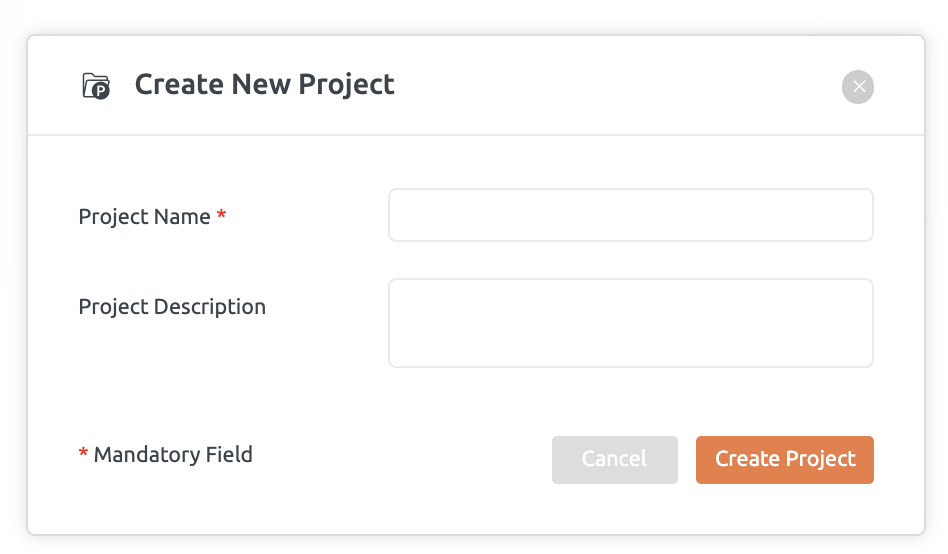
\includegraphics[width=4.5in, height=1.8in]{requirement.png}
\caption{User Requirement}
\label{fig:Requirement}
\end{center}
\end{figure}
The Embold Users have few more requirements about the code analysis, they would expect Embold to show them the result about the code issues, quality metrics, duplication, design and hotspots as well. These are pretty much functional requirements which Embold is fulfilling, as shown in Figure~\ref{fig:Requirement1}. \par
\begin{figure}[htbp]
\begin{center}
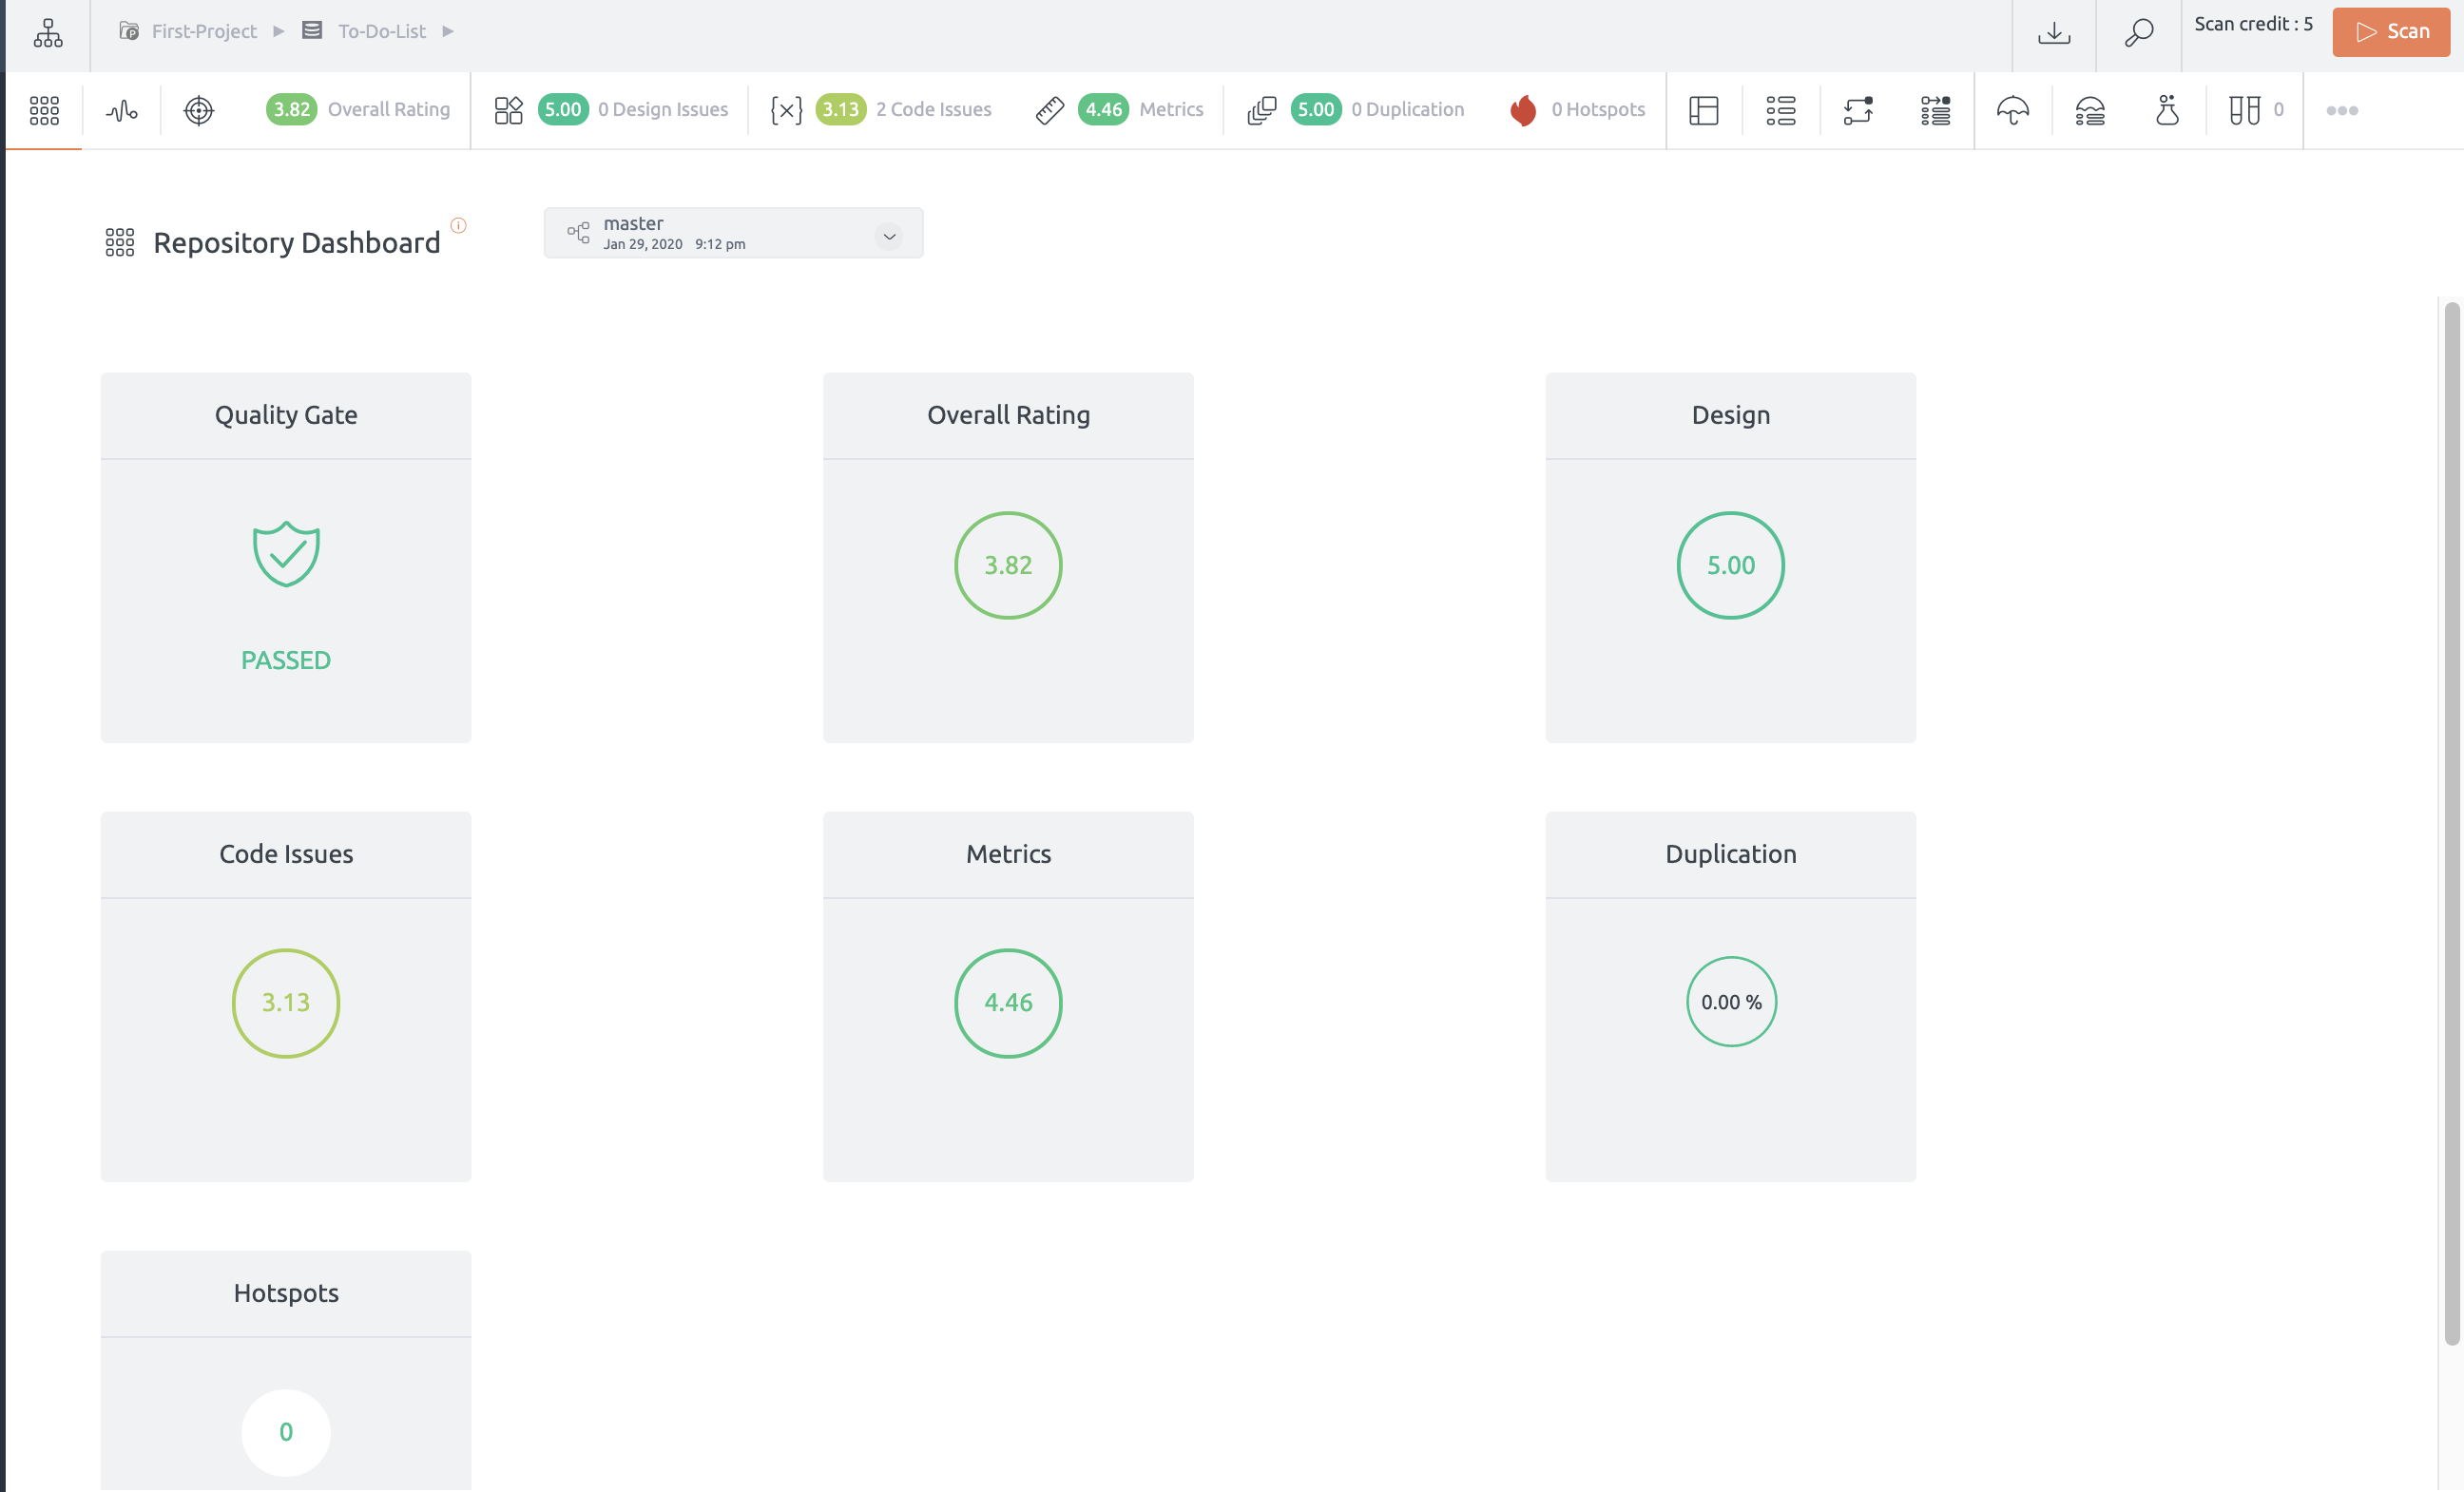
\includegraphics[width=6.5 in, height=3in]{requirement1.png}
\caption{User Requirement as an Output}
\label{fig:Requirement1}
\end{center}
\end{figure}
If we further delve into the output which we have in Figure~\ref{fig:Requirement1} we can notice that there are more detailed functionalities which are the important requirements of the user. More detail about code issues, metrics, hotspot etc as shown in Figure~\ref{fig:Requirement2}.\par
\begin{figure}[htbp]
\begin{center}
\includegraphics[width=6.5 in, height=3in]{requirement2.png}
\caption{User Requirement as Output in Detail}
\label{fig:Requirement2}
\end{center}
\end{figure}
Apart from all these the response time which the Embold takes to scan any project is also quite important. Embold also gives users to online help, info about price plans and also an ease to manage their profile using the options available in the profile as shown in Figure~\ref{fig:Requirement3}. All these are non-functional requirement which have a big impact on the product. 
\begin{figure}[htbp]
\begin{center}
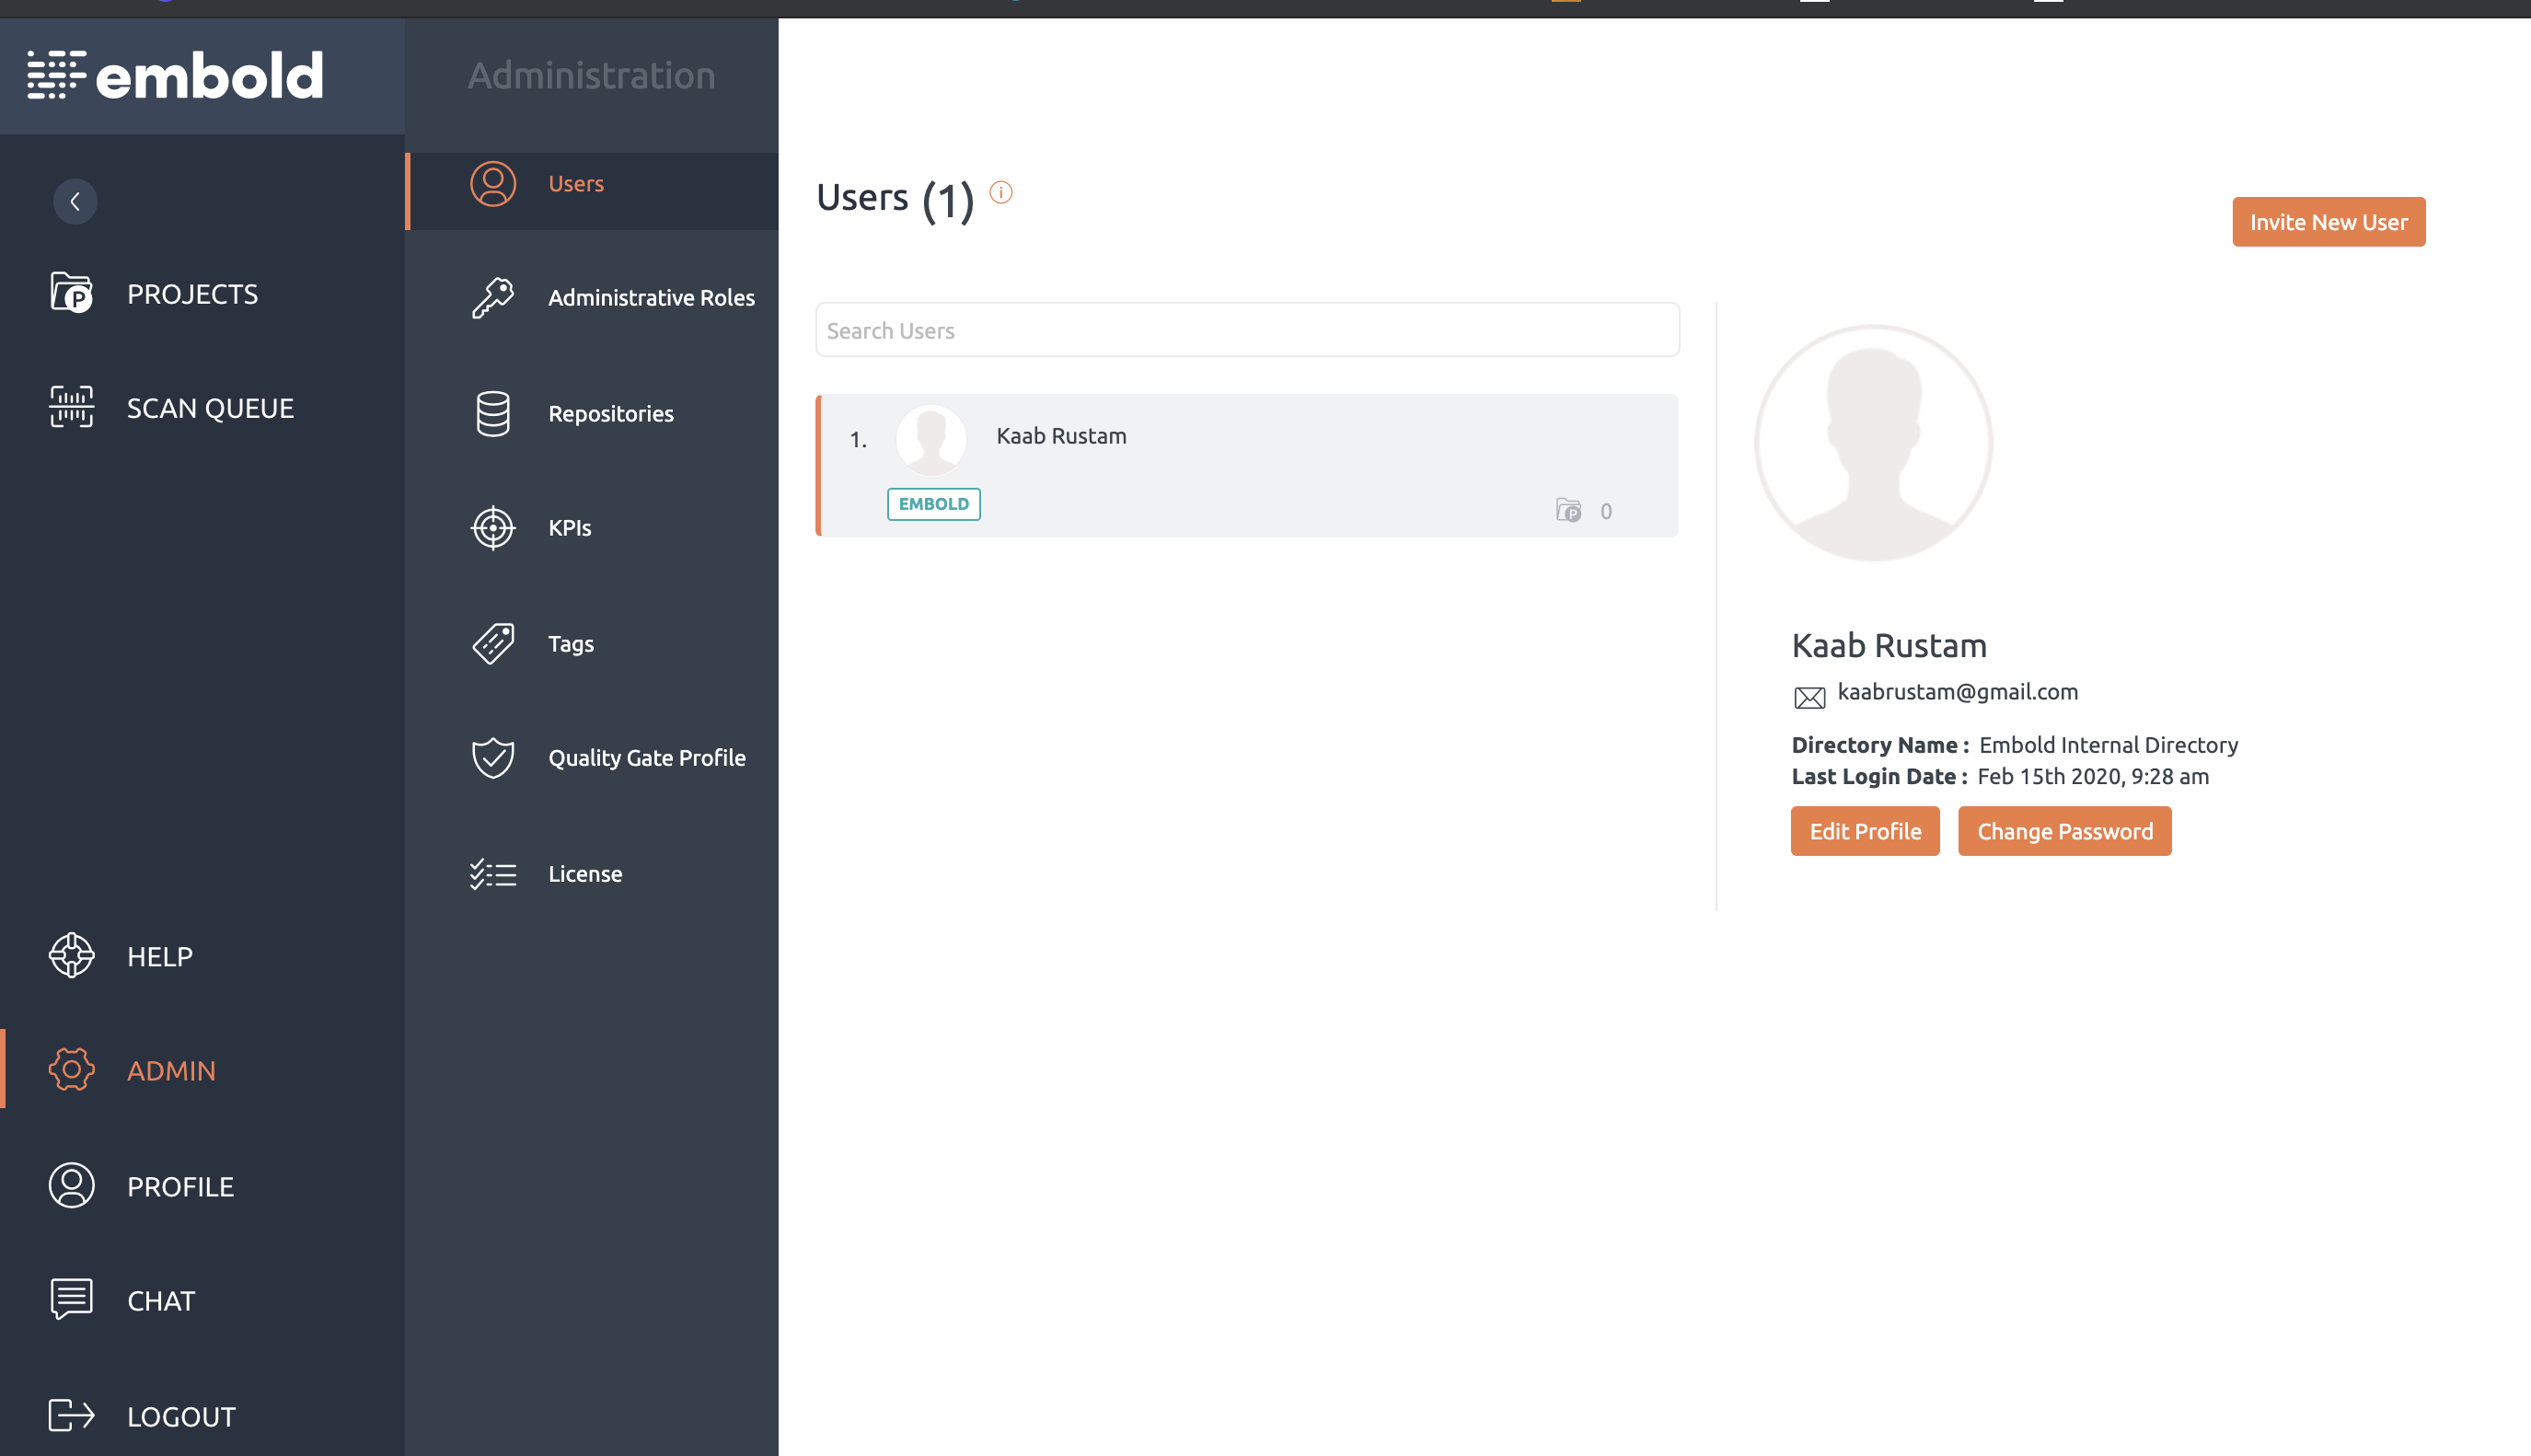
\includegraphics[width=6.5 in, height=3in]{Requirement3.png}
\caption{Non-functional Requirement example} 
\label{fig:Requirement3}
\end{center}
\end{figure}

